% Bản dịch tiếng Việt của paper/main.tex (commit 93f510d), dịch trung thành, để nhóm và mentor đọc.
% Bản nộp tạp chí là main.tex. Khi sửa main.tex phải sửa bản này theo.
% Số liệu dùng chung macro và bảng với main.tex (sinh tự động); số thập phân giữ dấu chấm như bản tiếng Anh.
% Biên dịch bằng XeLaTeX hoặc LuaLaTeX (cần fontspec cho tiếng Việt).
\documentclass[11pt]{article}
\usepackage[margin=1in]{geometry}
\usepackage{fontspec}
\usepackage[vietnamese]{babel}
\usepackage{amsmath,amssymb,booktabs,graphicx,xcolor,url,array}
\usepackage[hidelinks]{hyperref}
\newcommand{\todo}[1]{\textcolor{red}{[TODO: #1]}}
\renewcommand{\tablename}{Bảng}
\renewcommand{\figurename}{Hình}
\newcommand{\rqNgt}{135{,}275}
\newcommand{\rqRescuedOne}{9{,}909}
\newcommand{\rqStarvedOne}{63}
\newcommand{\rqRescuedEight}{10{,}141}
\newcommand{\rqStarvedEight}{82}
\newcommand{\rqRescuedTwo}{10{,}663}
\newcommand{\rqStarvedTwo}{42}
\newcommand{\rqZeroCandVtA}{19.8}

\newcommand{\dAvtAtwo}{+0.0090}
\newcommand{\dAvtAtwoSceneLo}{+0.0052}
\newcommand{\dAvtAtwoSceneHi}{+0.0149}
\newcommand{\dAvtAtwoCombLo}{$-$0.0088}
\newcommand{\dAvtAtwoCombHi}{+0.0269}
\newcommand{\nCombExcl}{0}
\newcommand{\gateCoef}{$-$0.33}
\newcommand{\gateLo}{$-$0.50}
\newcommand{\gateHi}{$-$0.16}
\newcommand{\recallZero}{6.5\%}
\newcommand{\recallOne}{33.5\%}
\newcommand{\recallFive}{53.2\%}

\newcommand{\pOneSFour}{+0.0085}
\newcommand{\pOneSFive}{+0.0087}
\newcommand{\pOneMean}{+0.0086}
\newcommand{\pOneAzeroSFour}{0.0430}
\newcommand{\pOneAtwoSFour}{0.0515}
\newcommand{\pOneOldMin}{+0.0045}
\newcommand{\pOneOldMax}{+0.0155}
\newcommand{\pOneNmsSFour}{+0.0081}
\newcommand{\pOneNmsSFive}{+0.0081}
\newcommand{\apNewMean}{+0.0039}
\newcommand{\apsNewMean}{$-$0.0014}
\newcommand{\apmNewMean}{$-$0.0083}
\newcommand{\apsOldMean}{$-$0.0043}
\newcommand{\apmOldMean}{$-$0.0083}
\newcommand{\rzeroDap}{+0.0015}
\newcommand{\rzeroDval}{$-$0.019}
\newcommand{\valCOne}{+0.133}
\newcommand{\valCOneN}{947}
\newcommand{\valLocShare}{69.7}
\newcommand{\valMissShare}{29.0}
\newcommand{\mOneOld}{+0.068}
\newcommand{\mOneNew}{+0.067}
\newcommand{\mOneOldLow}{+0.135}
\newcommand{\mOneNewLow}{+0.136}
\newcommand{\mOneSeedMin}{+0.062}
\newcommand{\mOneSeedMax}{+0.078}
\newcommand{\vtDetAzero}{24.8}
\newcommand{\vtDetAtwo}{30.2}
\newcommand{\vtMissAzero}{47.4}
\newcommand{\vtMissAtwo}{41.9}
\newcommand{\vtLocAzero}{27.5}
\newcommand{\vtLocAtwo}{27.6}
\newcommand{\vtMissShareUndet}{60.0}
\newcommand{\vtLocShareUndetLow}{65.0}
\newcommand{\vtMissShareUndetLow}{33.4}
\newcommand{\vtDetAtwoLow}{45.3}
\newcommand{\vtLocAtwoLow}{35.5}
\newcommand{\vtMissAtwoLow}{18.2}
\newcommand{\starvedAzero}{5.8}
\newcommand{\starvedAtwo}{16.4}
\newcommand{\fedAzero}{30.4}
\newcommand{\fedAtwo}{34.3}
\newcommand{\recVtOne}{78.4}
\newcommand{\recVtHalf}{45.3}
\newcommand{\recVtThreeQ}{4.7}
\newcommand{\dropVt}{19.6}
\newcommand{\dropT}{13.5}
\newcommand{\recVtHalfAzeroHigh}{24.8}
\newcommand{\recVtHalfAtwoHigh}{30.2}
\newcommand{\tStarvedAzero}{15.0}
\newcommand{\tStarvedAtwo}{30.7}
\newcommand{\tStarvedN}{1{,}166}
\newcommand{\didLogit}{+0.98}
\newcommand{\vtZeroCandTest}{22.8}
\newcommand{\nVtTest}{44{,}177}
\newcommand{\nScenesTest}{8{,}107}
\newcommand{\nScenesVt}{3{,}492}
\newcommand{\aTwoOldSd}{0.0062}
\newcommand{\apmNeg}{5}
\newcommand{\apmSeeds}{5}
\newcommand{\aZeroOldMax}{0.0415}
\newcommand{\aZeroNewMin}{0.0430}
\newcommand{\pOneNewApMax}{+0.0063}

\newcommand{\rtFrac}{31.4}
\newcommand{\oracleAP}{0.996}
\newcommand{\oracleVt}{0.998}
\newcommand{\lrZero}{0.01}
\newcommand{\momentum}{0.937}
\newcommand{\wDecay}{0.0005}
\newcommand{\warmup}{1}
\newcommand{\flipP}{0.5}
\newcommand{\envOldNumpy}{2.1.3}
\newcommand{\envOldPython}{3.13.15}
\newcommand{\envOldTorch}{2.11.0+cu130}
\newcommand{\envNewNumpy}{2.4.6}
\newcommand{\envNewPython}{3.13.16}
\newcommand{\envPhTwoTorch}{2.14.1+cu130}
\newcommand{\nposCoef}{+0.51}
\newcommand{\nposLo}{+0.38}
\newcommand{\nposHi}{+0.64}
\newcommand{\hTwoBFirst}{+0.270}
\newcommand{\hTwoBRest}{+0.142}
\newcommand{\medAtwoWo}{+0.167}
\newcommand{\medAtwoW}{$-$0.160}
\newcommand{\medAoneWo}{+0.169}
\newcommand{\medAoneW}{$-$0.038}
\newcommand{\medAeightWo}{+0.195}
\newcommand{\medAeightW}{+0.042}
\newcommand{\angPeakBin}{4--8}
\newcommand{\angSpread}{0.5}
\newcommand{\angPeak}{3.2}
\newcommand{\angSmall}{1.4}
\newcommand{\hOneBMeanAtwo}{$-$0.0020}


\begin{document}
\title{Sàn vùng ứng viên cho vật thể xoay rất nhỏ trong YOLO26n-OBB:\\ Một nghiên cứu thực nghiệm trên AI-TOD-R}
\author{Võ Đức Nhật, Trần Lợi Kiều Nhi, Trần Nguyễn Minh Hải, Nguyễn Tấn Tài\\ Đại học FPT, Việt Nam
\todo{Xác nhận thứ tự tác giả, cách viết tên (có dấu hay không dấu), đơn vị, email, và mentor có đứng tên không.}}
\date{}
\maketitle

\begin{abstract}
Trong các bộ phát hiện một giai đoạn (one-stage detector) chọn điểm neo ứng viên (candidate anchor) bằng cách kiểm tra tâm
điểm neo có nằm trong hộp nhãn thật (ground-truth box) hay không, một vật nhỏ hơn bước lưới đặc trưng (feature stride) có thể
không nhận được ứng viên nào, và do đó không có tín hiệu huấn luyện. Các bản YOLO gần đây của Ultralytics phóng to hộp nhỏ
trong bước chọn ứng viên để tránh điều này. Chúng tôi nghiên cứu quy tắc này cho hộp xoay (oriented box), dùng YOLO26n-OBB
trên phần không thuộc xView của AI-TOD-R. Trên nhãn huấn luyện, \rqZeroCandVtA\% hộp rất nhỏ ($<8$ px) không có điểm neo ứng
viên nào khi không có sàn (floor). Sàn của thư viện (A2: cạnh dưới 16 px được đặt bằng 16 px) và một sàn nhỏ hơn
$8\sqrt2$ px không để sót hộp nào. Chúng tôi so A2 với không có sàn (A0) trên ba seed huấn luyện thăm dò, và trên hai seed
tiếp theo theo một luật quyết định đã đăng ký trước (preregistered). AP$_{vt}$ tăng \pOneSFour{} và \pOneSFive{} trên hai seed
tiếp theo, từ mức khoảng 0.043. AP$_m$ giảm ở cả năm seed, còn AP tổng không thay đổi quá mức dao động giữa các seed. Các hộp
test rất nhỏ mà A0 sẽ để không có ứng viên được tăng recall từ sàn nhiều hơn các hộp rất nhỏ khác, thêm \mOneOld{} trên seed
1--3 và \mOneNew{} trên seed 4--5, nhưng phần lớn chúng vẫn không được phát hiện. Cách các hộp chưa được phát hiện chồng lên dự
đoán phụ thuộc mạnh vào ngưỡng score, nên dữ liệu không tách được định vị kém (localisation) với độ tin cậy thấp. Mọi kết quả
đến từ một mô hình nhỏ, một công thức huấn luyện 24 epoch và một tập con của một bộ dữ liệu.
\end{abstract}

\section{Giới thiệu}
Vật thể trong ảnh chụp từ trên cao thường chỉ rộng vài pixel. Trong AI-TOD-R, kích thước trung bình của vật khoảng 10.6 px
\cite{aitodr}, tương đương bước lưới nhỏ nhất của một kim tự tháp đặc trưng (feature pyramid). Gán nhãn căn chỉnh theo tác vụ
(task-aligned assignment) \cite{tood}, được các bộ phát hiện YOLO gần đây sử dụng, trước hết chỉ giữ làm ứng viên của một hộp
nhãn thật những điểm neo có tâm nằm trong hộp. Một hộp rơi vào khoảng giữa các tâm điểm neo sẽ không bao giờ là mẫu dương
(positive) của điểm neo nào và không đóng góp gì vào hàm mất mát (loss).

YOLO26 \cite{yolo26} xử lý vấn đề này bằng Gán nhãn nhận biết vật nhỏ (Small-Target-Aware Label Assignment, STAL): chỉ trong
bước chọn ứng viên, các cạnh hộp dưới một ngưỡng được thay bằng một giá trị lớn hơn, còn việc chấm điểm, gán mục tiêu và hồi
quy (regression) vẫn dùng hộp gốc. Thí nghiệm bóc tách (ablation) đã công bố được làm trên COCO với hộp ngang và báo một lần
chạy cho mỗi cấu hình \cite[Table~6]{yolo26}. Quy tắc dùng cho hộp xoay cũng đã thay đổi giữa các bản phát hành của thư viện:
không có sàn cho tới bản 8.4.7, cạnh dưới 8 px được đặt thành 16 px từ bản 8.4.8, và cạnh dưới 16 px được đặt thành 16 px từ
bản 8.4.128 \cite{ultralytics}.\footnote{Theo lịch sử phát hành của \texttt{ultralytics/utils/tal.py}; từ bản 8.4.8 đến 8.4.38,
sàn sửa trực tiếp hộp nhãn thật, lỗi này được sửa ở bản 8.4.39.} Vì vậy, kết quả báo cáo cho ``STAL'' phụ thuộc phiên bản
gói. Trong các bài được điểm ở Mục~2, chúng tôi không thấy đánh giá nào của quy tắc cho hộp xoay trên một bộ dữ liệu vật tí hon.

Ba câu hỏi tổ chức bài này. \textbf{RQ1}: bao nhiêu hộp xoay rất nhỏ không nhận được ứng viên nào khi không có sàn, và khi đã
áp sàn thì phần mất mẫu dương còn lại xảy ra ở đâu? \textbf{RQ2}: sàn của thư viện có làm tăng AP$_{vt}$ so với không có sàn trên
các seed huấn luyện không được dùng để chọn phép so sánh hay không, và nó tốn gì ở vật lớn hơn? \textbf{RQ3}: trên tập test, các
hộp rất nhỏ lẽ ra không có ứng viên có được tăng recall từ sàn nhiều hơn các hộp rất nhỏ khác không, và các hộp vẫn không được
phát hiện chồng lên dự đoán như thế nào?

Chúng tôi trả lời các câu hỏi này bằng thực nghiệm và không đề xuất bộ gán nhãn (assigner) mới. Từ nhãn huấn luyện, chúng tôi
đếm, cho mọi hộp và bốn quy tắc ứng viên, số ứng viên mỗi hộp nhận được. Bước này chính xác và tái tạo đúng mặt nạ ứng viên của
thư viện (Mục~\ref{sec:method}). Sau đó chúng tôi so sàn của thư viện với không có sàn trên năm seed huấn luyện, trong đó hai seed
cuối được huấn luyện sau khi một luật quyết định đăng ký trước đã được chốt (Mục~\ref{sec:rq2}). Cuối cùng, chúng tôi liên hệ hình
học ứng viên của từng hộp test với việc hộp đó có được phát hiện hay không (Mục~\ref{sec:rq3}). Nghiên cứu chỉ gồm một mô hình
nhỏ, một công thức huấn luyện và tập con không thuộc xView của một bộ dữ liệu, và Mục~\ref{sec:threats} liệt kê những gì điều
này không cho phép kết luận.

\section{Các công trình liên quan}
\textbf{Mẫu dương cho vật tí hon.} Nhiều hướng nghiên cứu quy điểm yếu của bộ phát hiện với vật tí hon về số mẫu dương ít ỏi
mà các vật này nhận được. RFLA \cite{rfla} và gán nhãn dựa trên NWD \cite{aitodv2} thay IoU bằng các thước đo thay đổi trơn với
độ lệch nhỏ. DCFL \cite{aitodr} gán nhãn động cho vật xoay tí hon và báo cáo, ở mức định tính, rằng chúng nhận ít mẫu dương hơn
vật lớn. Bảng benchmark AI-TOD-R của bài này không có bộ phát hiện họ YOLO. Các bộ gán nhãn gần đây hơn tăng hoặc xếp hạng lại
mẫu dương của vật tí hon: CDCEDet \cite{cdcedet} với anchor thích ứng theo tỉ lệ và ngưỡng IoU theo từng vật, đánh giá trên
AI-TOD-v2 và AI-TOD-R; DALA \cite{dala} với số mẫu dương thích ứng cho từng vật; NGLA \cite{ngla} với độ tương đồng Gauss và xếp
hạng theo chất lượng cho hộp ngang; và MFN-Net \cite{mfnnet} với gán nhãn linh hoạt trên SODA-A và AI-TOD. Các bài này đề xuất
bộ gán nhãn và báo cáo mức tăng độ chính xác. Chúng tôi thì lấy quy tắc đi kèm một bộ phát hiện thời gian thực được dùng rộng
rãi và theo dõi từng hộp qua quy tắc đó. \todo{Chưa đọc toàn văn CDCEDet, DALA và MFN-Net (mới có tóm tắt hoặc phần tóm tắt
của nhà xuất bản); NGLA đọc theo cấu trúc mục và tìm từ khóa. Cần xác nhận không bài nào có phân tích theo từng hộp như
Mục~\ref{sec:rq3}.}

\textbf{Vùng ứng viên rộng hơn hộp.} Mở rộng vùng lấy ứng viên không phải điều mới. FCOS \cite{fcos} lấy mẫu dương từ vùng tâm,
ATSS \cite{atss} chọn một số ứng viên cố định ở mỗi tầng kim tự tháp theo khoảng cách tới tâm, và YOLOX \cite{yolox} xét các
điểm neo trong một bán kính cố định quanh tâm hộp. OSCAR \cite{oscar} thay các mục tiêu hồng ngoại nhỏ hơn bước lưới bằng hộp
giả vuông với nhiều kích thước và thấy kích thước tốt nhất nằm ở giữa dải. Sàn kích thước trong bước chọn điểm-trong-hộp là
một thành viên đơn giản của họ phương pháp này. Đóng góp của chúng tôi không phải quy tắc, mà là các phép đo dạng đang được
dùng thực tế của nó trên hộp xoay rất nhỏ.

\textbf{Gán nhãn cho hộp xoay.} EARL \cite{earl}, SARFA-Net \cite{sarfa} và ARA \cite{ara} làm cho việc gán nhãn hộp xoay phụ
thuộc hình dạng hoặc tỉ lệ cạnh, trên các benchmark ảnh trên cao tổng quát. MCSA \cite{mcsa} nhắm tới vật xoay tí hon bằng cách
gán mẫu theo nhiều yếu tố trên nền RetinaNet-OBB, đánh giá trên DOTA và DIOR-R. \todo{ARA mới đọc ở mức tóm tắt.}

\textbf{Chẩn đoán lỗi bộ phát hiện.} Hoiem và cộng sự \cite{hoiem} và TIDE \cite{tide} quy lỗi phát hiện về các loại như định
vị, nhầm lớp và bỏ sót. Mục~\ref{sec:rq3} dùng một cách phân loại đơn giản hơn, xét theo từng hộp với IoU xoay, và không ước
lượng phần AP mất cho mỗi loại.

\section{Chọn ứng viên và sàn}\label{sec:method}
YOLO26-OBB đặt tâm điểm neo tại $((i+\tfrac12)s,(j+\tfrac12)s)$ trên ba tầng với bước lưới $s\in\{8,16,32\}$. Bộ gán nhãn căn
chỉnh theo tác vụ \cite{tood} của nó làm ba bước: (1) mọi điểm neo có tâm nằm trong hộp là ứng viên; (2) trong các ứng viên,
giữ $k$ ứng viên đứng đầu theo một thước đo căn chỉnh tính từ dự đoán của mô hình ($k=10$ cho nhánh một-nhiều (one-to-many);
$k=7$, rồi một, cho nhánh một-một (one-to-one) dùng khi suy luận); (3) một điểm neo được nhiều hộp giữ sẽ thuộc về hộp có độ
chồng lấn dự đoán cao nhất. Quy tắc sàn chỉ đổi bước (1): mỗi cạnh ngắn hơn $\tau$ được thay bằng $f$ trước phép kiểm nằm trong.
Chúng tôi nghiên cứu bốn quy tắc: A0, không có sàn; A1, $\tau=8$, $f=16$ (quy tắc STAL đã công bố); A8, $\tau=f=8\sqrt2$; và A2,
$\tau=f=16$ (quy tắc hiện tại của thư viện). Hình~\ref{fig:floor} cho thấy tác dụng trên một hộp.

\begin{figure}[t]\centering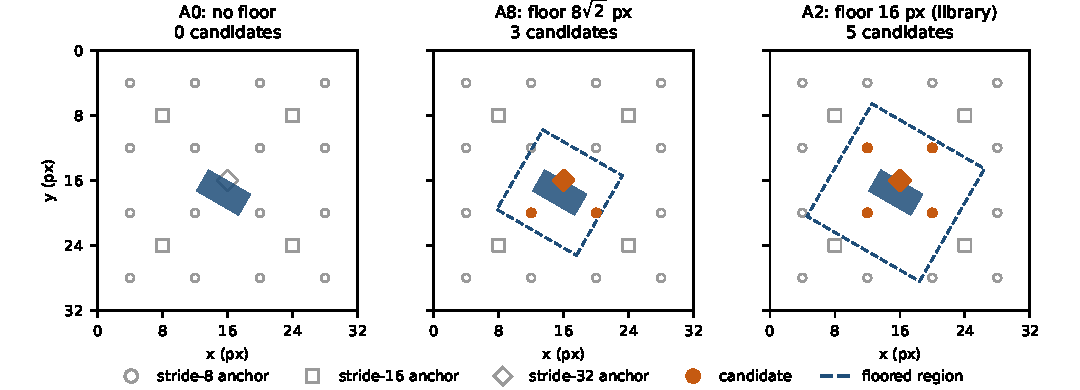
\includegraphics[width=\textwidth]{figs/floor_example}
\caption{Một hộp 6$\times$3 px xoay 30$^\circ$ không chứa tâm điểm neo nào (A0). Với sàn phủ tối thiểu (A8) nó nhận ba ứng viên,
và với sàn của thư viện (A2) là năm. Ứng viên tính bằng cùng mã với phân tích nhãn.}
\label{fig:floor}\end{figure}

Một hình chữ nhật xoay có cạnh ngắn ít nhất $\sqrt2\,s$ luôn chứa một điểm neo bước $s$ ở mọi vị trí và góc, vì lưới vuông
khoảng cách $s$ có bán kính phủ (covering radius) $s/\sqrt2$. Do đó A8 và A2 cho mọi hộp ít nhất một ứng viên. A1 thì không, vì
nó chỉ nâng các cạnh dưới 8 px. Điều này không nói gì về việc ứng viên có vượt qua bước (2) và (3) hay không, hoặc có giúp huấn
luyện hay không.

\textbf{Đếm chỉ từ nhãn.} Chúng tôi cài đặt bước (1) trên nhãn huấn luyện, và một kiểm thử đơn vị (unit test) xác nhận mặt nạ
ứng viên khớp với của thư viện trên các hộp ngẫu nhiên cho A0, A8 và A2. Bước (2) và (3) phụ thuộc dự đoán. Chúng tôi xấp xỉ
chúng bằng cách thay thước đo căn chỉnh bằng khoảng cách từ điểm neo tới tâm và gọi kết quả là phép xấp xỉ (proxy). Phép xấp
xỉ theo nhánh một-nhiều ($k=10$). Chúng tôi chưa so nó với kết quả gán nhãn được ghi lại trong lúc huấn luyện. Khi tắt mosaic,
co giãn và dịch chuyển, với đầu vào $800\times800$, phép lật ánh xạ lưới điểm neo lên chính nó, nên số đếm ở bước (1) đúng cho
mọi mẫu huấn luyện.

\textbf{Nhóm kích thước.} Chúng tôi dùng các nhóm của AITODReval trên $\sqrt{\text{diện tích}}$: rất nhỏ (very tiny) 2--8 px,
tí hon (tiny) 8--16 px, nhỏ (small) 16--32 px và trung bình (medium) 32--64 px.

\section{Thiết lập thực nghiệm}
\textbf{Dữ liệu.} AI-TOD-R \cite{aitodr} được dựng một phần từ ảnh xView, vốn cần đăng ký riêng mà chúng tôi không có. Chúng tôi
dùng ảnh từ các nguồn còn lại (woX): 8,426 ảnh huấn luyện, 936 ảnh kiểm định (validation) và 9,261 ảnh test. Ảnh kiểm định được
tách theo cảnh. Một cảnh gồm các ô cắt từ cùng một ảnh nguồn (một ô xView, một ảnh DOTA hoặc một khung hình VisDrone), và mỗi
ảnh khác là một cảnh riêng. Tập test có \nScenesTest{} cảnh, trong đó \nScenesVt{} cảnh chứa hộp rất nhỏ. Phép đếm chỉ từ nhãn
dùng các file nhãn woX còn ít nhất một hộp sau bộ lọc chính thức (cạnh $\geq 2$ px). Kết quả không so được với benchmark đầy đủ
của \cite{aitodr}.

\textbf{Huấn luyện.} YOLO26n-OBB \cite{yolo26} khởi tạo từ trọng số COCO, Ultralytics 8.4.174, 24 epoch, SGD với tốc độ học
\lrZero{} theo cách giảm mặc định của thư viện, momentum \momentum, weight decay \wDecay, \warmup{} epoch khởi động, batch 16, kích
thước đầu vào 800, lật ngang và lật dọc với xác suất \flipP, không tăng cường dữ liệu nào khác, độ chính xác hỗn hợp (mixed
precision), một GPU A100. Mosaic và co giãn ngẫu nhiên được bật mặc định trong Ultralytics. Chúng tôi tắt chúng để số đếm nhãn
giữ chính xác, nên công thức huấn luyện khác công thức mặc định. AP trên tập kiểm định vẫn đang tăng ở epoch 24. Benchmark trong
\cite{aitodr} huấn luyện 12 hoặc 40 epoch.

\textbf{Đánh giá.} Bộ chấm chính thức AITODReval giữ 1,500 phát hiện cho mỗi ảnh và lớp, nên chúng tôi đặt giới hạn của bộ phát
hiện là 12,000 cho mỗi ảnh. Đưa chính nhãn thật vào làm dự đoán cho AP \oracleAP{} và AP$_{vt}$ \oracleVt{}. Chúng tôi chấm
checkpoint cuối và báo riêng đầu một-một (e2e, mặc định khi suy luận của YOLO26) và đầu một-nhiều có NMS.

\textbf{Trình tự nghiên cứu.} Bảng~\ref{tab:sequence} liệt kê các bước theo thứ tự đã chạy và những gì đã được xem ở mỗi bước.
Mười hai lần chạy thăm dò (bốn quy tắc, seed 1--3) được chấm trên tập test trước khi bất kỳ luật nào được chốt. Từ đó chúng tôi
chọn phép so sánh A2 với A0 trên AP$_{vt}$ với đầu e2e, là cặp có chênh lệch thăm dò lớn nhất (\dAvtAtwo{}). Trước khi huấn luyện
seed 4 và 5, chúng tôi chốt một luật quyết định (P1): phép so sánh được coi là lặp lại được nếu $\Delta$AP$_{vt}>0$ trên cả hai
seed mới và trung bình của chúng ít nhất 0.006. Ngưỡng này là độ lệch chuẩn mẫu của AP$_{vt}$ của A2 trên seed 1--3
(\aTwoOldSd), đã làm tròn. Nó đo nhiễu giữa các seed và không được chọn vì ý nghĩa thực tế. Trong một mô phỏng ghi kèm bản đăng
ký trước, luật này tuyên bố lặp lại được trong khoảng 6.5\% trường hợp khi không có hiệu ứng. P1 là một luật quyết định, không
phải kiểm định ý nghĩa thống kê, và nó dùng lại chính các ảnh test đã dùng để chọn phép so sánh.

\begin{table}[t]\centering\caption{Trình tự nghiên cứu. Mỗi bước ghi những gì đã biết khi bước đó được chốt.}\label{tab:sequence}
\footnotesize\begin{tabular}{p{0.35\textwidth}p{0.55\textwidth}}\toprule
Bước & Đã xem trước bước này \\\midrule
1. Mười hai lần chạy thăm dò (A0, A1, A8, A2; seed 1--3), AP trên test & số ứng viên trên 300 file nhãn \\
2. Phân tích thăm dò 12 lần chạy: recall theo hộp trên tập kiểm định, phép kiểm số ứng viên, bootstrap & bước 1 \\
3. Đếm chỉ từ nhãn trên toàn bộ nhãn train+val và test & bước 1--2 \\
4. Số phận từng hộp trên ảnh kiểm định, 12 lần chạy; quyết định huấn luyện & bước 1--3 \\
5. Phụ lục đăng ký trước chốt P1, M1, M3 và các nhánh (A0, A2) & bước 1--4; chưa có kết quả theo hộp trên test \\
6. Seed 4--5 cho A0 và A2, lần chạy kiểm tái lập R0; AP trên test và phân tích theo hộp trên test & bước 1--5 \\\bottomrule
\end{tabular}\end{table}

\textbf{Kiểm tái lập.} Trước khi gộp seed 1--3 với seed 4--5, một lần chạy lại A2 seed 1 (R0) phải khớp bản gốc trong phạm vi
0.005 về AP trên test và về mAP kiểm định ở epoch 24. Các ngưỡng này được đặt khi phụ lục được chốt. Kế hoạch trước đó dùng 0.002
và 0.003 cho một đường mã huấn luyện khác.

\textbf{Phân tích theo từng hộp.} Một hộp test được tính là phát hiện được nếu một dự đoán cùng lớp có score ít nhất 0.25 khớp
với nó ở IoU xoay ít nhất 0.5, theo khớp tham lam (greedy matching) theo thứ tự score. Ngưỡng score 0.05 được báo để đối chiếu.
Một hộp chưa được phát hiện được gán kết quả đầu tiên phù hợp trong các loại sau: \emph{hàng xóm} (neighbour), một dự đoán cùng
lớp đạt IoU 0.5 với nó nhưng đã khớp với hộp khác; \emph{lớp} (class), một dự đoán khác lớp đạt IoU 0.5; \emph{định vị}
(localisation), dự đoán cùng lớp tốt nhất có IoU trong $[0.1, 0.5)$; \emph{cả hai} (both), dự đoán khác lớp tốt nhất có IoU trong
$[0.1, 0.5)$; \emph{bỏ sót} (missed), không dự đoán nào đạt IoU 0.1. Với hộp 4 px, một dự đoán lệch 3 px có thể có IoU bằng 0,
nên ``bỏ sót'' không có nghĩa là không có dự đoán nào ở gần. Chúng tôi chưa ước lượng tần suất IoU ít nhất 0.1 xảy ra do ngẫu
nhiên. M1 so mức tăng recall giữa hai nhóm hộp test rất nhỏ: các hộp mà hình học không cho ứng viên nào dưới A0 (``bị A0 bỏ
đói'', A0-starved; \vtZeroCandTest\% trong \nVtTest{} hộp test rất nhỏ) và các hộp còn lại. M1 là hiệu của hai hiệu recall A2$-$A0,
tính theo từng seed, và khoảng tin cậy của nó kết hợp bootstrap theo cụm cảnh ($B=10{,}000$) với dao động giữa các seed,
$\Delta\pm t_{0.975,n-1}\sqrt{\mathrm{se}_\text{cảnh}^2+\mathrm{se}_\text{seed}^2}$. Hộp test không được dùng để huấn luyện, nên
``bị A0 bỏ đói'' mô tả hình học của hộp, không phải lịch sử huấn luyện của nó.

\section{Kết quả và thảo luận}
\subsection{RQ1: khoảng một trong năm hộp rất nhỏ không có ứng viên khi không có sàn}\label{sec:rq1}
Bảng~\ref{tab:stages} đếm ứng viên cho \rqNgt{} hộp trong nhãn huấn luyện và kiểm định woX. Khi không có sàn, \rqZeroCandVtA\% hộp
rất nhỏ không có ứng viên (\vtZeroCandTest\% trên nhãn test). A8 và A2 loại bỏ phần mất mát này theo cấu tạo, còn A1 để sót một
phần rất nhỏ trong nhóm tí hon, làm tròn thành 0 trong bảng. Theo phép xấp xỉ cho bước (2) và (3), A2 đưa \rqRescuedTwo{} hộp từ
không có lên ít nhất một mẫu dương và \rqStarvedTwo{} hộp theo chiều ngược lại (A8: \rqRescuedEight{} và \rqStarvedEight{}; A1:
\rqRescuedOne{} và \rqStarvedOne{}). Các hộp vẫn không có mẫu dương dưới một sàn chủ yếu nằm trong cụm dày (Bảng~\ref{tab:density},
Hình~\ref{fig:stages}), nơi các vùng đã nâng sàn chồng lên nhau và điểm neo bị dùng chung. Mẫu hình theo mật độ này đến từ phép
xấp xỉ. Chúng tôi chưa kiểm nó trên đầu ra của bộ phát hiện, vì phép kiểm đã lên kế hoạch cần các lần chạy A8 mà không được huấn
luyện. \textbf{Trả lời RQ1:} khi không có sàn, khoảng một trong năm hộp rất nhỏ không nhận được ứng viên nào. Với A8 hoặc A2 thì
không hộp nào như vậy, và theo phép xấp xỉ, phần mất mẫu dương còn lại tập trung ở cụm dày.

\begin{table}[t]\centering\caption{Ứng viên và mẫu dương của mỗi hộp theo từng quy tắc, nhãn train+val woX. Mẫu dương dùng phép
xấp xỉ khoảng cách cho bước (2)--(3), nhánh một-nhiều. Nhãn hàng và cột trong các bảng số liệu giữ tiếng Anh như bản gốc; xem
Bảng~\ref{tab:glossary}.}\label{tab:stages}\footnotesize\begin{tabular}{lrrrr}
\toprule
 & A0 & A1 & A8 & A2 \\
\midrule
\multicolumn{5}{l}{\textit{very tiny ($<$8 px)}{,} $n=50{,}263$} \\
\quad candidates / GT & 1.04 & 3.79 & 2.61 & 5.37 \\
\quad zero candidates (\%) & 19.8 & 0.0 & 0.0 & 0.0 \\
\quad shared candidates (\%) & 5.1 & 44.9 & 34.5 & 50.6 \\
\quad zero positives, proxy (\%) & 20.7 & 2.7 & 2.4 & 1.4 \\
\multicolumn{5}{l}{\textit{tiny (8--16 px)}{,} $n=66{,}414$} \\
\quad candidates / GT & 2.92 & 4.18 & 3.82 & 5.98 \\
\quad zero candidates (\%) & 1.2 & 0.0 & 0.0 & 0.0 \\
\quad shared candidates (\%) & 7.3 & 18.3 & 13.8 & 27.5 \\
\quad zero positives, proxy (\%) & 1.5 & 0.3 & 0.2 & 0.1 \\
\multicolumn{5}{l}{\textit{small (16--32 px)}{,} $n=14{,}877$} \\
\quad candidates / GT & 10.31 & 10.34 & 10.42 & 11.43 \\
\quad zero candidates (\%) & 0.0 & 0.0 & 0.0 & 0.0 \\
\quad shared candidates (\%) & 9.3 & 9.8 & 9.7 & 13.1 \\
\quad zero positives, proxy (\%) & 0.0 & 0.0 & 0.0 & 0.0 \\
\bottomrule
\end{tabular}
\end{table}
\begin{table}[t]\centering\caption{Tỉ lệ hộp không có mẫu dương (xấp xỉ, \%) theo số tâm hộp khác trong bán kính 16 px: phần mất mát
còn lại dưới một sàn nằm ở cụm dày.}\label{tab:density}\footnotesize\begin{tabular}{llrrrrr}
\toprule
size & neighbours & $n$ & A0 & A1 & A8 & A2 \\
\midrule
very tiny & isolated & 13{,}765 & 18.2 & 0.0 & 0.0 & 0.0 \\
very tiny & 1--2 & 16{,}750 & 19.0 & 0.3 & 0.4 & 0.1 \\
very tiny & $\geq$3 & 19{,}748 & 23.9 & 6.7 & 5.7 & 3.4 \\
tiny & isolated & 31{,}841 & 1.0 & 0.0 & 0.0 & 0.0 \\
tiny & 1--2 & 27{,}898 & 1.4 & 0.1 & 0.1 & 0.1 \\
tiny & $\geq$3 & 6{,}675 & 4.3 & 2.1 & 1.9 & 1.2 \\
\bottomrule
\end{tabular}
\end{table}
\begin{figure}[t]\centering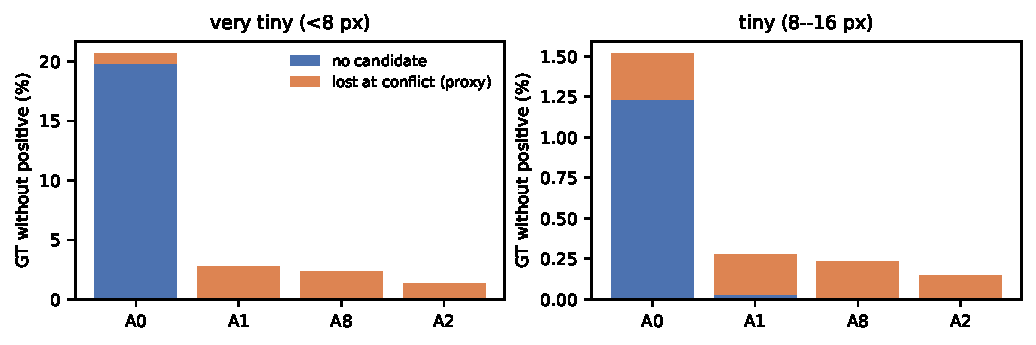
\includegraphics[width=0.75\textwidth]{figs/rq2_stages}
\caption{Hộp không có mẫu dương, chia thành hộp không có ứng viên (chính xác) và hộp mất mọi ứng viên khi xung đột (xấp xỉ).
Sàn loại bỏ phần thứ nhất.}\label{fig:stages}\end{figure}

\subsection{RQ2: sàn của thư viện làm tăng AP$_{vt}$ trên cả hai seed mới, và AP$_m$ giảm ở mọi seed}\label{sec:rq2}
Trên seed 4 và 5, $\Delta$AP$_{vt}$(A2$-$A0) là \pOneSFour{} và \pOneSFive{} (trung bình \pOneMean), nên P1 lặp lại được theo luật
(Bảng~\ref{tab:p1}). Mức nền thấp: A0 đạt AP$_{vt}$ \pOneAzeroSFour{} ở seed 4. Đầu NMS cho cùng chiều (\pOneNmsSFour{} và
\pOneNmsSFive). Trên seed 1--3, các chênh lệch nằm trong khoảng từ \pOneOldMin{} đến \pOneOldMax, và không khoảng thăm dò nào trong
40 khoảng có tính dao động seed loại được 0 (Phụ lục, Bảng~\ref{tab:explor}). Hai seed không cho được khoảng tin cậy hữu ích của
riêng chúng, nên kết quả dựa trên dấu và độ lớn của hai giá trị.

Sàn có cái giá ở vật lớn hơn. AP$_m$ dưới A2 thấp hơn ở \apmNeg{} trong \apmSeeds{} seed, và chênh lệch trung bình là \apmNewMean{} ở
mỗi nhóm seed, nhất quán giữa các seed không kém mức tăng AP$_{vt}$. AP$_s$ thay đổi \apsNewMean{} (seed 4--5) và \apsOldMean{} (seed
1--3), với dấu không đồng nhất. AP tổng thay đổi \apNewMean{} trung bình trên seed 4--5, dưới hiệu ứng tối thiểu 0.005 đặt cho AP,
và mọi khoảng tin cậy của nó đều chứa 0. Sàn 16 px phóng to vùng ứng viên của mọi hộp nhỏ hơn kích thước đó, điều này có thể kéo
điểm neo khỏi các vật lớn hơn ở gần. Chúng tôi chưa kiểm cách giải thích này.

Lần chạy kiểm tái lập không khớp. AP trên test chênh \rzeroDap, trong ngưỡng, nhưng mAP kiểm định ở epoch 24 chênh \rzeroDval,
ngoài ngưỡng. Các lần chạy A0 của seed 4--5 cũng có AP$_{vt}$ cao hơn (từ \aZeroNewMin) mọi lần chạy A0 của seed 1--3 (cao nhất
\aZeroOldMax). Cả hai đều cho thấy môi trường huấn luyện đã thay đổi giữa hai nhóm lần chạy (Phụ lục~\ref{app:env}). Phép so sánh
trong seed 4--5 vẫn là so cặp, nhưng được thực hiện trong một môi trường khác với các lần chạy thăm dò, và hai nhóm được báo cáo
riêng. \textbf{Trả lời RQ2:} trong điều kiện này, sàn của thư viện làm tăng AP$_{vt}$ khoảng 0.009 trên cả hai seed mới, không làm
AP tổng thay đổi có thể phát hiện được, và làm giảm AP$_m$.

\begin{table}[t]\centering\caption{AP trên test theo từng seed, đầu e2e. $\Delta$ là A2 trừ A0. Seed 1--3 đã được xem trước khi
chốt P1; seed 4--5 được huấn luyện sau đó, trong một môi trường khác (Mục~\ref{sec:rq2}).}\label{tab:p1}\scriptsize
\begin{tabular}{llrrrrrrr}
\toprule
Seeds & Seed & AP$_{vt}$ A0 & AP$_{vt}$ A2 & $\Delta$AP$_{vt}$ & $\Delta$AP$_t$ & $\Delta$AP$_s$ & $\Delta$AP$_m$ & $\Delta$AP \\
\midrule
1--3, exploratory & 1 & 0.0411 & 0.0456 & +0.0045 & +0.0071 & $-$0.0112 & $-$0.0074 & +0.0009 \\
 & 2 & 0.0415 & 0.0570 & +0.0155 & +0.0074 & +0.0109 & $-$0.0042 & +0.0083 \\
 & 3 & 0.0401 & 0.0472 & +0.0070 & +0.0042 & $-$0.0125 & $-$0.0132 & +0.0014 \\
 & mean & & & +0.0090 & +0.0062 & $-$0.0043 & $-$0.0083 & +0.0035 \\
\midrule
4--5, new & 4 & 0.0430 & 0.0515 & +0.0085 & +0.0077 & $-$0.0009 & $-$0.0028 & +0.0063 \\
 & 5 & 0.0430 & 0.0518 & +0.0087 & +0.0048 & $-$0.0018 & $-$0.0138 & +0.0014 \\
 & mean & & & +0.0086 & +0.0063 & $-$0.0014 & $-$0.0083 & +0.0039 \\
\bottomrule
\end{tabular}
\end{table}

\subsection{RQ3: hộp bị A0 bỏ đói được lợi nhiều nhất trong các hộp rất nhỏ, nhưng phần lớn vẫn không được phát hiện}\label{sec:rq3}
Các hộp test rất nhỏ mà A0 để không có ứng viên được tăng recall dưới A2 nhiều hơn các hộp rất nhỏ khác (Bảng~\ref{tab:m1}):
\mOneOld{} trên seed 1--3 và \mOneNew{} trên seed 4--5 ở score $\geq 0.25$, và \mOneOldLow{} và \mOneNewLow{} ở score $\geq 0.05$ (hiệu
recall ghi dạng tỉ số). Cả năm giá trị theo seed ở score $\geq 0.25$ đều dương (từ \mOneSeedMin{} đến \mOneSeedMax). Tiêu chí đã đăng
ký trước cho M1 đòi một khoảng kết hợp không chứa 0. Điều này đạt trên seed 1--3, vốn là thăm dò và có kết quả tương ứng trên tập
kiểm định đã được xem. Trên seed 4--5 khoảng tin cậy chứa 0, nên M1 không được ủng hộ ở đó theo chính tiêu chí của nó. Trên thang
logit, chênh lệch là \didLogit{} (trung bình trên seed 1--5), có tính tới việc nhóm bị bỏ đói xuất phát từ recall thấp hơn nhiều.
Hai nhóm còn khác nhau về kích thước, tỉ lệ cạnh và lớp trong nhóm rất nhỏ, và chúng tôi chưa kiểm soát các yếu tố này.

Mức tăng không biến hộp bị A0 bỏ đói thành hộp được phát hiện. Ở score $\geq 0.25$, \starvedAtwo\% các hộp này được phát hiện dưới
A2, so với \starvedAzero\% dưới A0, trong khi các hộp rất nhỏ khác đạt \fedAtwo\% (\fedAzero\% dưới A0). Một số hộp bị A0 bỏ đói vẫn
được phát hiện dù không có ứng viên, gợi ý rằng dự đoán từ các điểm neo lân cận có thể phủ được chúng. Trong nhóm tí hon (8--16 px),
\tStarvedN{} hộp bị A0 bỏ đói tăng từ \tStarvedAzero\% lên \tStarvedAtwo\% được phát hiện, mức tăng lớn hơn so với nhóm rất nhỏ.

Bảng~\ref{tab:fates} và Hình~\ref{fig:iou} mô tả các hộp chưa được phát hiện. Ở score $\geq 0.25$, A2 phát hiện \vtDetAtwo\% hộp rất
nhỏ so với \vtDetAzero\% của A0; tỉ lệ xếp vào bỏ sót giảm (\vtMissAtwo\% so với \vtMissAzero\%) và tỉ lệ xếp vào định vị giữ
nguyên (\vtLocAtwo\% và \vtLocAzero\%). Bỏ sót khi đó là kết quả lớn nhất trong các hộp rất nhỏ chưa được phát hiện
(\vtMissShareUndet\%). Ở score $\geq 0.05$ bức tranh đảo ngược: định vị là kết quả lớn nhất (\vtLocShareUndetLow\% so với
\vtMissShareUndetLow\% bỏ sót), và mức tăng của A2 chủ yếu lấy từ nhóm định vị. Vì vậy, nhiều hộp bị tính là bỏ sót ở ngưỡng cao
hơn thực ra có một dự đoán điểm thấp với độ chồng lấn nhất định. Recall của hộp rất nhỏ dưới A2 ở score $\geq 0.05$ giảm từ
\recVtOne\% ở IoU 0.1 xuống \recVtHalf\% ở IoU 0.5 và \recVtThreeQ\% ở 0.75. Mức giảm từ IoU 0.25 xuống 0.5 (score $\geq 0.25$) là
\dropVt{} điểm với hộp rất nhỏ và \dropT{} điểm với hộp tí hon. Lệch một hai pixel là một phần lớn của hộp dưới 8 px, đó cũng là
động cơ của các thước đo dựa trên khoảng cách cho vật tí hon \cite{aitodv2}. Các bảng này là trung bình trên seed 1--5 và mang
tính mô tả. \todo{Tạo lại Bảng~\ref{tab:fates} và Hình~\ref{fig:iou} riêng cho seed 1--3 và 4--5 từ các file theo seed trên Drive
của nhóm.}

\textbf{Trả lời RQ3:} các hộp mà A0 sẽ bỏ đói được tăng recall từ sàn nhiều hơn các hộp rất nhỏ khác ở mọi seed, nhưng chưa tới
một phần năm số đó được phát hiện dưới A2. Với dữ liệu này, không tách được các hộp rất nhỏ còn lại thất bại do định vị hay do
score thấp: câu trả lời đổi theo ngưỡng score, và sàn cũng thay đổi điểm neo nào hồi quy mỗi hộp.

\begin{table}[t]\centering\caption{M1: hiệu của hiệu recall, A2$-$A0, hộp test bị A0 bỏ đói trừ các hộp rất nhỏ khác, đầu e2e. Khoảng
kết hợp cho seed 4--5 dùng $t$ với một bậc tự do.}\label{tab:m1}\footnotesize\begin{tabular}{llrcc}
\toprule
Score & Seeds & DiD & Scene 95\% CI & Scene + seed 95\% CI \\
\midrule
$\geq 0.25$ & 1--3 & +0.068 & [+0.055, +0.080] & [+0.033, +0.103] \\
 & 4--5 & +0.067 & [+0.054, +0.078] & [$-$0.023, +0.157] \\
$\geq 0.05$ & 1--3 & +0.135 & [+0.116, +0.152] & [+0.093, +0.177] \\
 & 4--5 & +0.136 & [+0.118, +0.154] & [$-$0.004, +0.277] \\
\bottomrule
\end{tabular}
\end{table}
\begin{table}[t]\centering\caption{Kết quả của các hộp test, \% số hộp trong nhóm kích thước, đầu e2e, trung bình trên seed 1--5. Loại
kết quả chiếm ưu thế trong các hộp rất nhỏ chưa được phát hiện phụ thuộc ngưỡng score.}\label{tab:fates}\scriptsize
\begin{tabular}{lllrrrrrr}
\toprule
Score & Size & Arm & detected & neighbour & class & localisation & both & missed \\
\midrule
$\geq 0.25$ & very tiny & A0 & 24.8 & 0.0 & 0.1 & 27.5 & 0.3 & 47.4 \\
 &  & A2 & 30.2 & 0.0 & 0.1 & 27.6 & 0.3 & 41.9 \\
 & tiny & A0 & 53.9 & 0.2 & 0.2 & 18.9 & 0.2 & 26.6 \\
 &  & A2 & 57.0 & 0.2 & 0.2 & 18.7 & 0.2 & 23.8 \\
\midrule
$\geq 0.05$ & very tiny & A0 & 39.2 & 0.0 & 0.2 & 39.3 & 0.8 & 20.6 \\
 &  & A2 & 45.3 & 0.0 & 0.2 & 35.5 & 0.7 & 18.2 \\
 & tiny & A0 & 68.1 & 0.1 & 0.3 & 20.6 & 0.4 & 10.4 \\
 &  & A2 & 69.3 & 0.1 & 0.3 & 19.8 & 0.4 & 10.1 \\
\bottomrule
\end{tabular}
\end{table}
\begin{figure}[t]\centering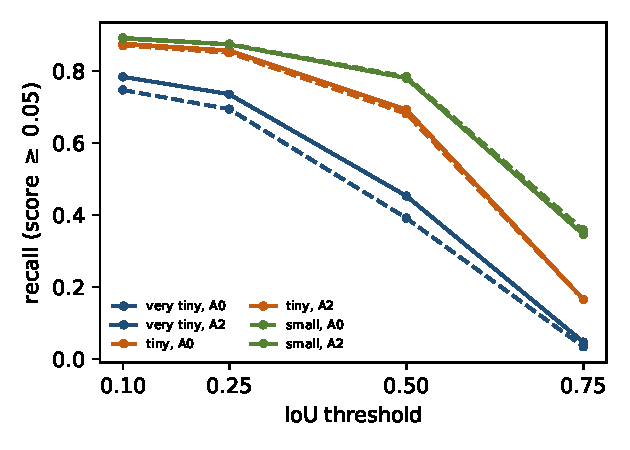
\includegraphics[width=0.6\textwidth]{figs/recall_iou}
\caption{Recall theo ngưỡng IoU, score $\geq 0.05$, đầu e2e, trung bình trên seed 1--5. Hộp rất nhỏ mất phần lớn recall giữa IoU 0.25
và 0.5.}\label{fig:iou}\end{figure}

\subsection{Các giả thuyết đã đăng ký trước khác}\label{sec:other}
Bảng~\ref{tab:prereg} ở Phụ lục liệt kê mọi giả thuyết cùng kết quả. Tất cả đã chạy trước khi bản đăng ký trước được merge và là
thăm dò. Hai kết quả liên quan tới cơ chế. Thứ nhất, trên ảnh kiểm định, recall của hộp dưới 8 px tăng theo số mẫu dương được gán
ở checkpoint cuối (hệ số \nposCoef, CI 95\% [\nposLo, \nposHi]; \recallZero{} khi không có, \recallOne{} khi có một, \recallFive{} khi có
năm đến chín), nhưng quan hệ này có thể theo cả hai chiều, vì cách chọn căn chỉnh theo tác vụ ưu tiên các hộp mà mô hình đã dự đoán
tốt. Thứ hai, phép kiểm số ứng viên đã lên kế hoạch, vốn chỉ phụ thuộc hình học, cho hệ số âm (\gateCoef, CI 95\% [\gateLo, \gateHi])
sau khi kiểm soát kích thước, tỉ lệ cạnh, độ dày đặc và lớp. Chúng tôi chưa giải thích được dấu âm này. Trong cùng một nhánh và nhóm
kích thước, số ứng viên chủ yếu thay đổi theo vị trí của hộp trên lưới điểm neo. Kết quả này khiến chúng tôi bỏ một sàn thích ứng
đã lên kế hoạch. Sai số góc trung vị không giảm đều theo kích thước: nó cao nhất với hộp \angPeakBin{} px (\angPeak$^\circ$ với A0) và
chênh nhau tối đa \angSpread$^\circ$ giữa các quy tắc.

\subsection{Các mối đe dọa đến tính hợp lệ}\label{sec:threats}
Phép so sánh A2 với A0 được chọn trên chính các ảnh test mà sau đó dùng để đánh giá nó. Chỉ có các seed huấn luyện là mới. Hai nhóm
seed được huấn luyện trong các môi trường khác nhau, và phép kiểm tái lập thất bại ở mAP kiểm định. Các bảng theo từng hộp lấy trung
bình cả năm seed dù các nhóm không được gộp ở chỗ khác. Mô hình là biến thể nhỏ nhất của YOLO26, huấn luyện 24 epoch không có
mosaic hay tăng cường co giãn, trên phần không thuộc xView của một bộ dữ liệu. Sàn có thể hoạt động khác khi huấn luyện lâu hơn, khi
có tăng cường làm thay đổi kích thước hộp, hoặc với mô hình lớn hơn. Phép xấp xỉ cho bước gán nhãn (2) và (3) chưa được so với kết
quả gán nhãn ghi lại khi huấn luyện, và nó theo nhánh một-nhiều trong khi kết quả chính dùng đầu một-một. Hai nhóm của M1 khác nhau
về kích thước, tỉ lệ cạnh và lớp. Các loại kết quả dùng ngưỡng IoU cố định và khớp tham lam, không phải cách khớp của bộ chấm, và
không có mức cơ sở ngẫu nhiên. Nhãn của các hộp vài pixel có nhiễu: chuyển đa giác chính thức sang hộp xoay rồi chuyển ngược lại
chỉ tái tạo được \rtFrac\% số hộp ở IoU ít nhất 0.999. Trong quá trình nghiên cứu, các file đánh giá NMS của tám lần chạy thăm dò bị
mất khỏi bộ nhớ dùng chung. Các file của A2 seed 1--3 được dựng lại từ bộ nhớ đệm đánh giá gốc, chỉ ảnh hưởng tới số liệu của đầu NMS.
Một kiểm thử đơn vị cho đường chấm nhanh, vốn đã chấm seed 4--5 trong đợt đầu khi kiểm thử còn qua, bị lỗi trong môi trường phân
tích thứ hai và được bỏ qua ở đó.

\section{Kết luận}
Với các hộp xoay rất nhỏ trong phần không thuộc xView của AI-TOD-R, YOLO26n-OBB không có sàn ứng viên để khoảng một trong năm hộp
không có ứng viên nào. Sàn của thư viện cho mọi hộp một ứng viên, làm tăng AP$_{vt}$ khoảng 0.009 trên hai seed mới, giữ AP tổng
không đổi trong mức dao động giữa các seed và làm giảm AP$_m$ ở mọi seed. Các hộp được sàn cứu khỏi tình trạng không có ứng viên
được tăng recall nhiều nhất trong các hộp rất nhỏ, nhưng phần lớn vẫn không được phát hiện, và với dữ liệu hiện có chúng tôi
không thể nói định vị hay độ tin cậy giới hạn chúng nhiều hơn. Các bước tiếp theo xuất phát từ những thiếu sót nêu trên: huấn
luyện sàn phủ tối thiểu A8 trên seed mới, tách các bảng theo hộp theo nhóm seed, kiểm soát kích thước hộp và lớp trong phép so
sánh theo hộp, và lặp lại nghiên cứu với huấn luyện lâu hơn, tăng cường dữ liệu tiêu chuẩn và một bộ dữ liệu thứ hai.

\section*{Khả năng tái lập}
Bản đăng ký trước, mã phân tích, notebook và file kết quả: \url{https://github.com/VoDucNhatku/nckh-group7-tiny-obb}
(\texttt{experiments/}, \texttt{scripts/rq2/}, \texttt{scripts/c11x/}). Mã huấn luyện và đánh giá \texttt{scripts/c11/}:
\todo{công khai}. Trọng số mô hình và dự đoán dạng DOTA: \todo{link phát hành}.

\appendix
\section{Các giả thuyết đã đăng ký trước}\label{app:prereg}
\begin{table}[h]\centering\caption{Mọi giả thuyết đã đăng ký trước và kết quả. Các mục H chạy trên mười hai lần chạy thăm dò trước
khi bản đăng ký trước được merge và là thăm dò; H2b và H2c dùng ảnh kiểm định và đầu NMS; P1 và các mục M theo phụ lục chốt trước
seed 4--5 (M1 và M3 dùng seed 1--5 trên test).}\label{tab:prereg}\scriptsize
\begin{tabular}{lp{6.2cm}p{6.2cm}}
\toprule
Mã & Dự báo & Kết quả \\
\midrule
H1a & $\Delta$AP$_{vt}>0$ cho A1, A8, A2 so với A0, cả hai đầu & đúng (mô tả) \\
H1b & mức tăng do sàn ở đầu NMS lớn hơn ở đầu e2e & không được ủng hộ: 0 trên 3 nhánh đạt luật \\
H1c & $\Delta$AP$_s\leq 0$ với các sàn, cả hai đầu & đúng (mô tả) \\
H2a & recall tăng theo số ứng viên (cổng) & không được ủng hộ: hệ số âm \\
H2b & mẫu dương đầu tiên quan trọng nhất với hộp $<8$ px & đúng một phần: +0.270 so với +0.142; chưa tính tỉ lệ 95\% \\
H2c & hiệu ứng của nhánh giảm $\geq 50\%$ khi đưa mẫu dương vào & đúng với A1, A8; không đúng với A2 \\
H3a--c & các lần chạy K-floor & hủy sau cổng \\
H4a & sai số góc giảm theo kích thước & không được ủng hộ: cao nhất ở 4--8 px \\
H4b & các nhánh lệch nhau trong 2$^\circ$ ở cùng kích thước & đúng (lệch tối đa 0.5$^\circ$) \\
P1 & $\Delta$AP$_{vt}$(A2$-$A0) $>0$ trên seed 4, 5, trung bình $\geq 0.006$ & lặp lại được theo luật \\
M1 & hộp bị bỏ đói trừ hộp rất nhỏ khác, $\Delta$recall $>0$ & dương ở mọi seed; đạt tiêu chí trên seed 1--3, không đạt trên 4--5 \\
M2 & A2$-$A8 lớn hơn ở cụm dày & hủy (không huấn luyện A8) \\
M3a & bỏ sót là kết quả lớn nhất (A2, rất nhỏ) & đúng ở score $\geq 0.25$; đảo ngược ở $\geq 0.05$ \\
M3b & hộp bị bỏ đói vẫn có recall thấp hơn dưới A2 & đúng \\
M3c & mức giảm IoU 0.25$\to$0.5 ở hộp rất nhỏ lớn hơn ở hộp tí hon & đúng (đã thấy trên tập kiểm định trước) \\
\bottomrule
\end{tabular}
\end{table}

Với H2c, hệ số của A2 so với A0 trong mô hình recall đổi từ \medAtwoWo{} sang \medAtwoW{} khi đưa số mẫu dương vào, nên dấu đổi chiều
và hệ số không co về 0. Với A1 nó đổi từ \medAoneWo{} sang \medAoneW{} và với A8 từ \medAeightWo{} sang \medAeightW.

\section{Các phép so sánh thăm dò}\label{app:explor}
\begin{table}[h]\centering\caption{Seed 1--3, test woX. Scene: chỉ bootstrap theo cụm cảnh. Scene + seed: khoảng kết hợp với $t$ hai
bậc tự do.}\label{tab:explor}\scriptsize\begin{tabular}{llrcc}
\toprule
Head & Pair and metric & $\Delta$ & Scene 95\% CI & Scene + seed 95\% CI \\
\midrule
e2e & A1$-$A0, AP$_{vt}$ & +0.0074 & [+0.0032, +0.0158] & [$-$0.0094, +0.0243] \\
e2e & A1$-$A0, AP$_{t}$ & +0.0016 & [$-$0.0006, +0.0032] & [$-$0.0056, +0.0088] \\
e2e & A1$-$A0, AP$_{s}$ & $-$0.0064 & [$-$0.0102, $-$0.0034] & [$-$0.0200, +0.0073] \\
e2e & A1$-$A0, AP$_{m}$ & $-$0.0022 & [$-$0.0089, +0.0058] & [$-$0.0227, +0.0182] \\
e2e & A1$-$A0, AP & +0.0006 & [$-$0.0009, +0.0024] & [$-$0.0074, +0.0087] \\
e2e & A8$-$A0, AP$_{vt}$ & +0.0071 & [+0.0000, +0.0115] & [$-$0.0089, +0.0230] \\
e2e & A8$-$A0, AP$_{t}$ & +0.0042 & [+0.0006, +0.0073] & [$-$0.0082, +0.0167] \\
e2e & A8$-$A0, AP$_{s}$ & $-$0.0026 & [$-$0.0068, +0.0005] & [$-$0.0180, +0.0127] \\
e2e & A8$-$A0, AP$_{m}$ & $-$0.0029 & [$-$0.0086, +0.0044] & [$-$0.0321, +0.0263] \\
e2e & A8$-$A0, AP & +0.0025 & [+0.0005, +0.0047] & [$-$0.0105, +0.0155] \\
e2e & A2$-$A0, AP$_{vt}$ & +0.0090 & [+0.0052, +0.0149] & [$-$0.0088, +0.0269] \\
e2e & A2$-$A0, AP$_{t}$ & +0.0062 & [+0.0041, +0.0082] & [$-$0.0001, +0.0126] \\
e2e & A2$-$A0, AP$_{s}$ & $-$0.0043 & [$-$0.0088, $-$0.0003] & [$-$0.0383, +0.0297] \\
e2e & A2$-$A0, AP$_{m}$ & $-$0.0083 & [$-$0.0168, $-$0.0010] & [$-$0.0290, +0.0125] \\
e2e & A2$-$A0, AP & +0.0035 & [+0.0017, +0.0056] & [$-$0.0076, +0.0147] \\
e2e & A2$-$A8, AP$_{vt}$ & +0.0019 & [$-$0.0033, +0.0118] & [$-$0.0228, +0.0267] \\
e2e & A2$-$A8, AP$_{t}$ & +0.0020 & [$-$0.0010, +0.0055] & [$-$0.0141, +0.0181] \\
e2e & A2$-$A8, AP$_{s}$ & $-$0.0016 & [$-$0.0049, +0.0021] & [$-$0.0389, +0.0357] \\
e2e & A2$-$A8, AP$_{m}$ & $-$0.0054 & [$-$0.0139, +0.0006] & [$-$0.0449, +0.0341] \\
e2e & A2$-$A8, AP & +0.0011 & [$-$0.0010, +0.0032] & [$-$0.0180, +0.0201] \\
\midrule
nms & A1$-$A0, AP$_{vt}$ & +0.0065 & [+0.0034, +0.0127] & [$-$0.0124, +0.0255] \\
nms & A1$-$A0, AP$_{t}$ & +0.0013 & [$-$0.0014, +0.0033] & [$-$0.0097, +0.0122] \\
nms & A1$-$A0, AP$_{s}$ & $-$0.0066 & [$-$0.0106, $-$0.0031] & [$-$0.0311, +0.0178] \\
nms & A1$-$A0, AP$_{m}$ & $-$0.0069 & [$-$0.0143, +0.0022] & [$-$0.0252, +0.0113] \\
nms & A1$-$A0, AP & +0.0002 & [$-$0.0018, +0.0020] & [$-$0.0086, +0.0089] \\
nms & A8$-$A0, AP$_{vt}$ & +0.0057 & [$-$0.0004, +0.0089] & [$-$0.0074, +0.0188] \\
nms & A8$-$A0, AP$_{t}$ & +0.0037 & [$-$0.0002, +0.0067] & [$-$0.0094, +0.0167] \\
nms & A8$-$A0, AP$_{s}$ & $-$0.0045 & [$-$0.0083, $-$0.0013] & [$-$0.0180, +0.0089] \\
nms & A8$-$A0, AP$_{m}$ & $-$0.0087 & [$-$0.0151, $-$0.0014] & [$-$0.0293, +0.0120] \\
nms & A8$-$A0, AP & +0.0015 & [$-$0.0006, +0.0037] & [$-$0.0104, +0.0134] \\
nms & A2$-$A0, AP$_{vt}$ & +0.0071 & [+0.0028, +0.0150] & [$-$0.0083, +0.0224] \\
nms & A2$-$A0, AP$_{t}$ & +0.0047 & [+0.0018, +0.0070] & [$-$0.0020, +0.0113] \\
nms & A2$-$A0, AP$_{s}$ & $-$0.0095 & [$-$0.0133, $-$0.0049] & [$-$0.0340, +0.0150] \\
nms & A2$-$A0, AP$_{m}$ & $-$0.0102 & [$-$0.0196, $-$0.0011] & [$-$0.0347, +0.0143] \\
nms & A2$-$A0, AP & +0.0010 & [$-$0.0012, +0.0033] & [$-$0.0070, +0.0090] \\
nms & A2$-$A8, AP$_{vt}$ & +0.0013 & [$-$0.0039, +0.0121] & [$-$0.0182, +0.0209] \\
nms & A2$-$A8, AP$_{t}$ & +0.0010 & [$-$0.0013, +0.0036] & [$-$0.0084, +0.0104] \\
nms & A2$-$A8, AP$_{s}$ & $-$0.0050 & [$-$0.0079, $-$0.0009] & [$-$0.0263, +0.0164] \\
nms & A2$-$A8, AP$_{m}$ & $-$0.0015 & [$-$0.0092, +0.0054] & [$-$0.0331, +0.0300] \\
nms & A2$-$A8, AP & $-$0.0005 & [$-$0.0023, +0.0013] & [$-$0.0118, +0.0108] \\
\bottomrule
\end{tabular}
\end{table}

\section{Môi trường phần mềm}\label{app:env}
Các lần chạy thăm dò: Python \envOldPython, numpy \envOldNumpy, torch \envOldTorch. Seed 4--5 và R0: Python \envNewPython, numpy
\envNewNumpy, cùng torch và Ultralytics 8.4.174. Đợt phân tích thứ hai chạy với torch \envPhTwoTorch. Mọi lần chạy dùng một GPU
NVIDIA A100.

\section{Thuật ngữ}\label{app:glossary}
\begin{table}[h]\centering\caption{Thuật ngữ dùng trong bản dịch.}\label{tab:glossary}\footnotesize
\begin{tabular}{p{0.3\textwidth}p{0.25\textwidth}p{0.35\textwidth}}\toprule
Tiếng Anh & Bản dịch & Giải thích ngắn \\\midrule
candidate anchor & điểm neo ứng viên & điểm neo được xét làm mẫu dương của một hộp \\
candidate floor & sàn vùng ứng viên & kích thước tối thiểu của hộp khi chọn ứng viên \\
ground-truth box & hộp nhãn thật & hộp do người gán nhãn \\
positive sample & mẫu dương & điểm neo được dùng để học một vật \\
feature stride & bước lưới đặc trưng & khoảng cách giữa hai tâm điểm neo trên một tầng \\
task-aligned assignment & gán nhãn căn chỉnh theo tác vụ & cách gán của TOOD, dựa trên điểm phân loại và IoU \\
one-to-many / one-to-one & một-nhiều / một-một & nhánh gán nhiều hoặc đúng một điểm neo cho mỗi vật \\
proxy & phép xấp xỉ & ước lượng bước (2)--(3) chỉ từ nhãn \\
very tiny / tiny & rất nhỏ / tí hon & nhóm 2--8 px và 8--16 px theo $\sqrt{\text{diện tích}}$ \\
scene & cảnh & các ô cắt từ cùng một ảnh nguồn \\
A0-starved & bị A0 bỏ đói & hộp không có ứng viên nào khi không có sàn \\
localisation & định vị & dự đoán cùng lớp có IoU từ 0.1 đến dưới 0.5 \\
preregistration & đăng ký trước & chốt giả thuyết và luật trước khi xem dữ liệu \\
covering radius & bán kính phủ & khoảng cách xa nhất từ một điểm tới điểm lưới gần nhất \\
reproducibility check & kiểm tái lập & chạy lại một lần chạy cũ để so kết quả \\\bottomrule
\end{tabular}\end{table}

\bibliographystyle{unsrt}
\bibliography{refs}
\end{document}
